\documentclass[12pt]{article}

\usepackage[margin=1in]{geometry} 
\usepackage{amsmath,amsthm,amssymb}
\usepackage[spanish]{babel}
\usepackage[utf8]{inputenc}
\usepackage{tikz-cd}
\usepackage{amsmath}
\usepackage[shortlabels]{enumitem}
\usepackage{mathtools}
\usepackage{float}

\usepackage{afterpage}

\newcommand\blankpage{%
    \null
    \thispagestyle{empty}%
    \addtocounter{page}{-1}%
    \newpage}

\title{SWAP: Ejercicio T4.1}
\author{
        Antonio Gámiz Delgado
}

\begin{document}
\maketitle

Vamos a comparar un mainframe con una granja web en términos de coste y potencia. 

Para el mainframe vamos a enfocarnos en el z15 de IBM, que nos da elegir entre varias opciones de hardware (Max34,..., Max190). Vamos a elegir la más básica, Max34, que viene con:

\begin{itemize}
\item CPU: 34 cores 5.2GHz
\item 40TB RAIM
\end{itemize}

Este mainframe nos saldría por unos 250000 doláres.

Para la granja web vamos a seleccionar 102 Raspberry Pi 4 modelo B (59,95 euros por unidad) , con las siguientes especificaciones:

\begin{itemize}
\item CPU: Broadcom BCM2711 Cortex-A72 1,5GHz Quad-Core 64bits
\item RAM: 4GB LPDDR4-2400 SDRAM
\item: Memoria adicional: ninguna
\end{itemize}

He elegido el triple de Raspberry Pi por intentar compensar la diferencia en la frecuencia de los procesadores. Más 40 discuos duros SSD de 1TB, que nos saldría a 108,89 euros la unidad. En total la granja web nos saldría por unos 10470 euros.

Vemos claramente que la granja web sale mucho más barato. De hecho, buscando información para este ejercicio, he encontrado artículos donde el escritor se preguntaba por qué IBM seguía incluso frabicando mainframes.
\medskip

\begin{thebibliography}{9}
\bibitem{ibmpage} 
Página de IBM
https://www.ibm.com/es-es/it-infrastructure/servers/mainframes

\bibitem{descripcionz15}
Z15
https://www.ibm.com/es-es/marketplace/z15/resources,

\bibitem{z15hardware}
Z15 hardware
https://www.ibm.com/downloads/cas/NN7GBPJ1

\bibitem{raspberrry}
Raspberrypi hardware
https://www.tiendatec.es/raspberry-pi/placas-base/1100-raspberry-pi-4-modelo-b-4gb-765756931182.html?src=raspberrypi

\bibitem{precioz15}
Precio z15 https://www.zdnet.com/article/ibm-launches-z15-mainframe-aims-to-automate-compliance-via-data-privacy-passports/

\bibitem{preciossd}
Precio SSD
https://www.amazon.es/disco-duro-ssd-1tb/s?k=disco+duro+ssd+1tb

\end{thebibliography}
%\begin{figure}[H]
%  \center
%  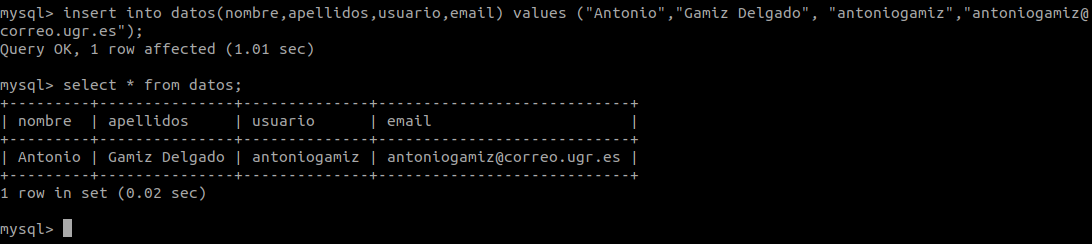
\includegraphics[scale=0.5]{img/3.png}
%\end{figure}

\end{document}
